\documentclass{beamer}
\usepackage[french]{babel}
\usepackage{float}
\usepackage[T1]{fontenc}
\usepackage{hyperref}
\usepackage[utf8]{inputenc}

\title{Présentation du sujet de simulation et contrôle d'écoulements instables par intelligence artificielle}
\author{julien VALENTIN}
\date{Juin 2022}

\begin{document}

\maketitle

\begin{frame}{Introduction}
    \begin{itemize}
    \setlength\itemsep{1.5em}
        \item CNAM
        \item ONERA
        \item programme Artificial Intelligence for Health, Physics, Transportation and Defense
            \begin{itemize}
                \item 4 axes de recherche
                \item 10 doctorants
                \item durée de 3 ans
            \end{itemize}
        \item cofinancé par l'ANR
    \end{itemize}
\end{frame}

\begin{frame}{Ma formation initiale (1/2)}
    \begin{itemize}
    \setlength\itemsep{1.15em}
        \item lycée et C.P.G.E en sciences de l'ingénieur
        \item un an à CentraleSupélec, campus de Metz
        \item bifurcation licence de maths/physique à Sorbonne-Université
        \item projet de fin de licence sur l'algorithme DeepTexture de Léon Gatys
    \end{itemize}
\end{frame}

\begin{frame}{Ma formation initiale (2/2)}
    \begin{itemize}
    \setlength\itemsep{1.15em}
    \item ouverture à l'Observatoire de Paris (12 ECTS en Master 1)
    \item master de mathématique spécialité mathématiques de la modélisation, Sorbonne-Université.
    \item stage de fin d'étude à l'Institut de Mathématique de Marseille : analyse numérique par volumes finis sur maillage M.A.C structuré des équations de Stokes, Darcy et Brinkman auprès de Philippe Angot
    \end{itemize}
\end{frame}

\begin{frame}{Depuis l'obtention du diplôme}
\begin{columns}[t]
    \begin{column}{0.49\textwidth}
        \centering
        \textbf{Ingénieur R\&D}
        \vspace{15pt}
        \begin{itemize}
            \item TENSYL SARL, PME à Périgny (17)
            \item Modélisation et simulation de procédés de fabrications de matériaux composites
            \item Problèmes multiphysiques (écoulements, poreux, structure, thermique)
            \item Problèmes multi-échelle : matériau, mèche, fibre
            \item FreeFEM++
        \end{itemize}
    \end{column}
    \begin{column}{0.49\textwidth}
        \centering
        \textbf{Enseignant vacataire bac +3}
        \vspace{15pt}
        \begin{itemize}
            \item EPITA, Paris
            \item $12 \times 2$ heures
            \item Travaux Pratiques d'algèbre numérique
            \item Python : Pandas, Numpy, Scipy
            \item PCA, Resolution de systemes lineaires, conditionnement et pré-conditionnement, SVD...
        \end{itemize}
    \end{column}
\end{columns}
\end{frame}

\begin{frame}{Présentation générale du sujet de thèse}
    \begin{figure}
    \centering
        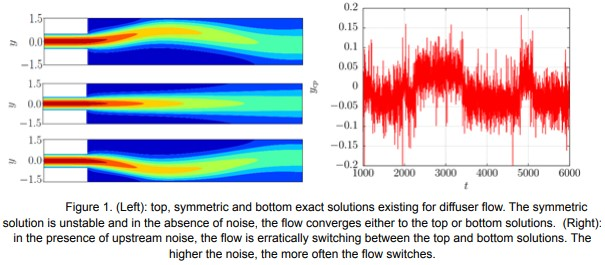
\includegraphics[height=.35\textheight]{images/phenomene_bistable.jpg}
    \end{figure}
    \vspace{20pt}
    \begin{columns}
        \begin{column}{0.49\textwidth}
            \centering
            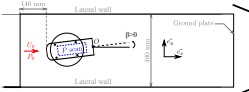
\includegraphics[width = \textwidth]{images/dispositif_bifurcation_experimental.jpg}
        \end{column}
        \begin{column}{0.49\textwidth}
            \centering
            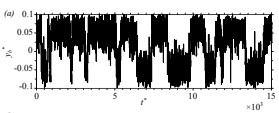
\includegraphics[width = \textwidth]{images/barycentre_pression_bifurcation_experimental.jpg}
        \end{column}
    \end{columns}
\end{frame}

\begin{frame}{Simulation des écoulements (1/5)}{Stokes après obstacle}
    \begin{equation*}
        \left\{
        \begin{array}{rcl}
        \nabla \cdot u & = & 0 \\
        -\nu \Delta u + \nabla p & = & 0
        \end{array}
        \right.
    \end{equation*}
    \begin{figure}
    \centering
        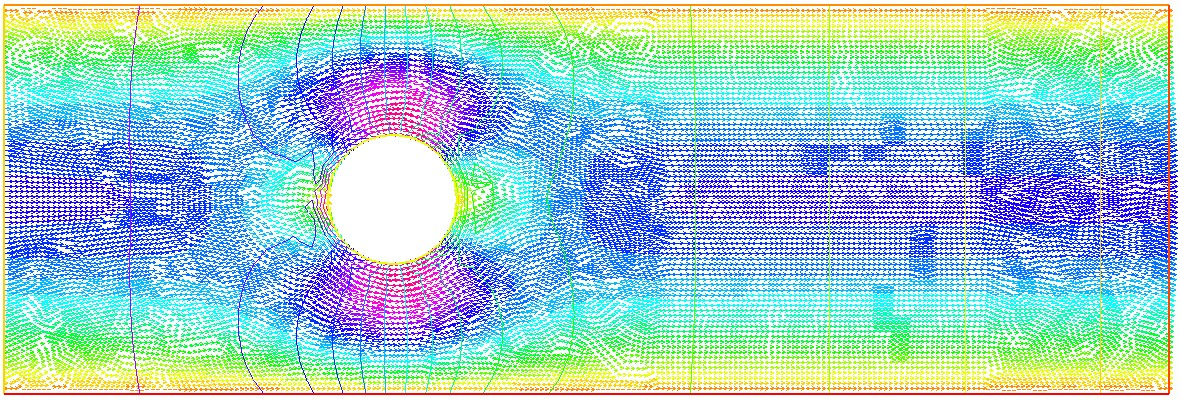
\includegraphics[width=\textwidth]{images/stokes_obstacle_centre.jpg}
        \caption{Setup point-selle d'un lagrangien, éléments finis de Taylor-Hood P2/P1, conditions aux limites de Poiseuille et stabilisation de la pression}
    \end{figure}
\end{frame}

\begin{frame}{Simulation des écoulements (2/5)}{Stokes en cavité entraînée}
    \begin{figure}
    \centering
        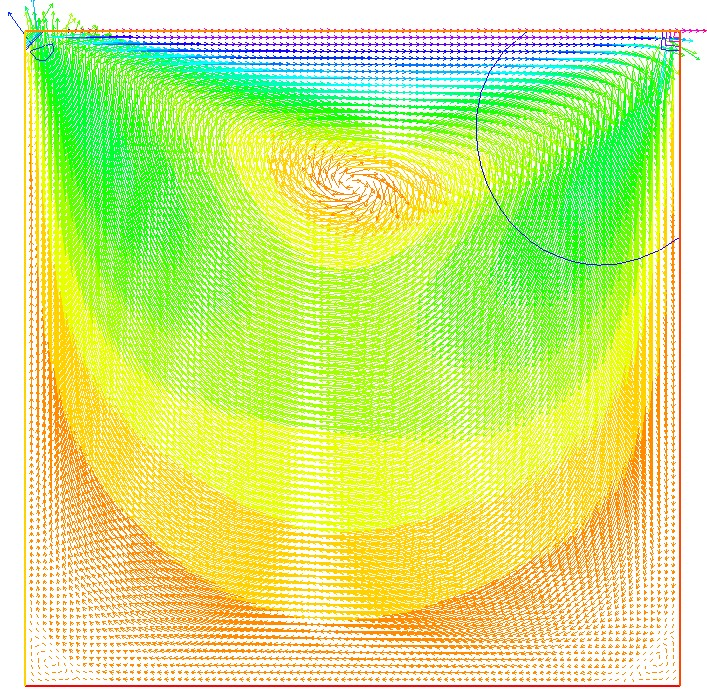
\includegraphics[scale=.30]{images/stokes_cavite_uzawa.jpg}
        \caption{Schéma d'Uzawa pour le lagrangien augmenté, éléments finis de Taylor-Hood P2/P1, conditions aux limites de vitesse pour la cavité entraînée}
    \end{figure}
\end{frame}

\begin{frame}{Simulation des écoulements (3/5)}{Navier-Stokes après obstacle}
    \begin{equation*}
        \left\{
        \begin{array}{rcl}
        \nabla \cdot u & = & 0 \\
        \partial_t u + (u\cdot\nabla)u & = & \nu \Delta u - \nabla p
        \end{array}
        \right.
        \hspace{20pt} w := \partial_y u^x - \partial_x u^y
    \end{equation*}
    \begin{figure}
    \centering
        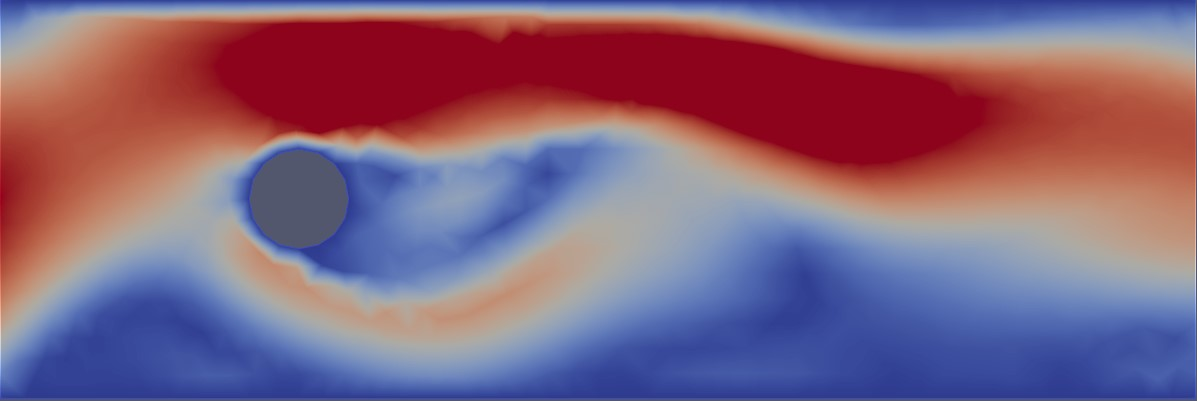
\includegraphics[height=.30\textheight]{images/navierStokes_obstacle_vitesse.jpg}
    \end{figure}
    \begin{figure}
    \centering
        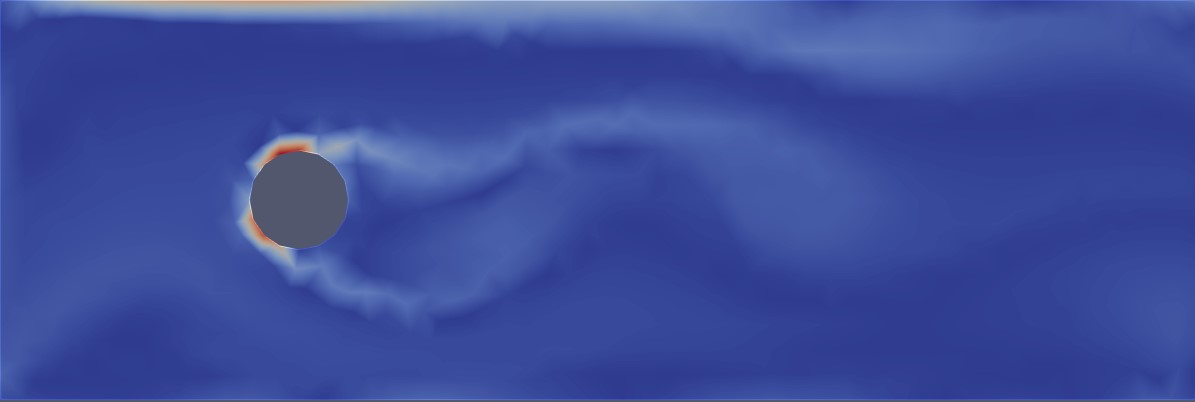
\includegraphics[height=.30\textheight]{images/navierStokes_obstacle_vortex.jpg}
    \end{figure}
\end{frame}

\begin{frame}{Simulation des écoulements 4/5}{Méthode basée sur l'apprentissage statistique}
    \begin{itemize}
        \item méthode de Décomposition Orhogonale aux valeurs Propres (POD) : on considère une suite finie de solutions $(U_i)$, appelées \emph{snapshoots}, et on cherche une base orthogonale $(\psi_j)$ d'interpolation qui minimise l'erreur sur l'ensemble des $U_i$. Pour $d$ modes : $$ \text{argmin}_{\{\psi_j\}} \frac{1}{L} \sum_{i=1}^{L} \left\| U_i - \sum_{j=1}^{d} (U_i|\psi_j) \psi_j \right\|^2 $$
    \end{itemize}
\end{frame}

\begin{frame}{Simulation des écoulements 5/5}{Autres méthodes d'apprentissage statistique}
    \begin{itemize}
        \item méthodes de Décomposition Dynamique en Modes : trouver un opérateur linéaire $A$ tel que la suite $(A^i U_0)_i$ minimise l'erreur des moindres carrés
        
        \item méthodes de Physics-informed Neural Networks : on ajoute à la fonction de coût usuelle la contribution de la norme du résidu
        $$ J : W, b \mapsto \frac{1}{L_u} \sum_{i=1}^{L_u} \| u(t_u^i, x_u^i) - u^i \|^2 + \frac{1}{L_f} \sum_{i=1}^{L_f} \| f(t_f^i, x_f^i) \|^2 $$
        où $f$ est un schéma pour le membre de gauche.
    \end{itemize}
\end{frame}

\begin{frame}{Apprentissage par renforcement}{Framework}
    \begin{figure}
    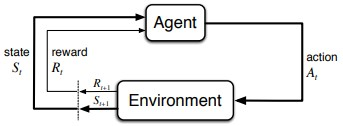
\includegraphics[]{images/framework_reinforcement_learning.jpg}
    \end{figure}
    \begin{align*}
        \mathbf{g} & := \nabla_\theta \mathbb{E} \left[ \gamma^t r_t \right] \\
        \mathcal{L}_\theta & := -\frac{1}{L} \sum_{i=1}^{L} A^\pi(s_i, a_i) \text{ln}( \pi^\theta(a_i|s_i) )
    \end{align*}
\end{frame}

\begin{frame}{Conclusion}
    \begin{itemize}
    \setlength\itemsep{1.15em}
        \item Langage Python3, avec API MPI, PETSc, FEniCs, frameworks de machine-learning...
        \item simulations par éléments finis : FEniCs/dolfinx (API PETSc)
        \item framework pour l'apprentissage statistique en général : Scikit-learn
        \item implémentation de l'environnement : openAI/Gym
        \item framework pour le deep-learning : Tensorflow, Pytorch
    \end{itemize}
    \vspace{15pt}
    Autre langage pour le machine-learning : Julia. \\
    \vspace{15pt}
    Autre langage de haut niveau pour les éléments finis : FreeFEM++.
\end{frame}

\begin{frame}{Sur l'étagère...}
\begin{thebibliography}{5}
    \bibitem{textbook}
        Pierre Saramito (2016) \emph{Complex fluids
        Modeling and Algorithms}, \href{https://membres-ljk.imag.fr/Pierre.Saramito/rheolef/html/index.html}{\underline{site internet de Rheolef}}
    \bibitem{textbook}
        N. Thuerey, P. Holl, M. Mueller, P. Schnell, F. Trost, K. Um (2021) \emph{Physics-based Deep Learning}, \href{https://physicsbaseddeeplearning.org/}{\underline{site internet du livre}}
    \bibitem{texbook}
        Richard S. Sutton, Andrew G. Barto (2018) \emph{Reinforcement Learning:
        An Introduction}, The MIT Press
    \bibitem{texbook}
        Tarik Fahlaoui (2020) \emph{Réduction de modèles et apprentissage de solutions
spatio-temporelles paramétrées à partir de données :
application à des couplages EDP-EDO}, PhD Thesis.
    \bibitem{textbook}
    Antoine Dumon (2011) \emph{Réduction dimensionnelle de type PGD pour la résolution des écoulements incompressibles}, PhD Thesis.
\end{thebibliography}
    et quelques réalisations et recherches personnelles sur \href{https://github.com/julienVLNT/python-sandbox/tree/main/machine\%20learning}{\underline{ma page github}}
\end{frame}

\begin{frame}{Annexe : Singular Value Decomposition}
    Soit une matrice de données $X$ telle que le nombre d'attributs est grand devant le nombre d'observations $$ X := \left. \begin{pmatrix} \vdots & \vdots & \cdots & \vdots \\ x^1 & x^2 & \dots & x^m \\ \vdots & \vdots & \dots & \vdots \end{pmatrix} \right\} n \; \text{features} $$
    On appelle décomposition en valeurs singulières de $X$ l'unique triplet $(U, \Sigma, V)$ tel que $U \in \mathcal{M
    }_{n \times n}(\mathbb{R})$, $\Sigma \in \mathcal{M}_{n \times m}$ diagonale par blocs et $V \in \mathcal{M}_{m \times m}$ tel que
    \begin{equation*}
        X = 
        \begin{bmatrix} 
            \vdots & \vdots & \cdots & \vdots \\
            u^1    & u^2    & \dots  & u^n    \\ 
            \vdots & \vdots & \dots & \vdots
        \end{bmatrix}
        \begin{bmatrix}
            \sigma_1 & & & \\
            & \sigma_2 & & \\
            & & \ddots &   \\
            & & & \sigma_m \\
            \hline
            & & (0) & &
        \end{bmatrix}
        \begin{bmatrix}
            \vdots & \vdots & \cdots & \vdots \\
            v^1    & v^2    & \dots  & v^m    \\ 
            \vdots & \vdots & \dots & \vdots
        \end{bmatrix}^T
    \end{equation*}
\end{frame}

\begin{frame}{Annexe : décomposition D.M.D}
    On obtient un premier exemple de décomposition dynamique en modes en considérant les deux matrices de données 
    $$ X := \begin{pmatrix} \vdots & \vdots & \cdots & \vdots \\ x^1 & x^2 & \dots & x^{N_t-1} \\ \vdots & \vdots & \dots & \vdots \end{pmatrix} \;\;\;\; X' := \begin{pmatrix} \vdots & \vdots & \cdots & \vdots \\ x^2 & x^3 & \dots & x^{N_t} \\ \vdots & \vdots & \dots & \vdots \end{pmatrix} $$ On cherche $A$ telle que $X' \sim A X$. La matrice
    \begin{equation*}
        A := X' V \Sigma^{-1} U^T
    \end{equation*}
    où apparaît la S.V.D de X convient.
\end{frame}

\begin{frame}{Annexe : Réseau de neurones profonds}{dense, séquentiel}
    \begin{figure}
    \centering
        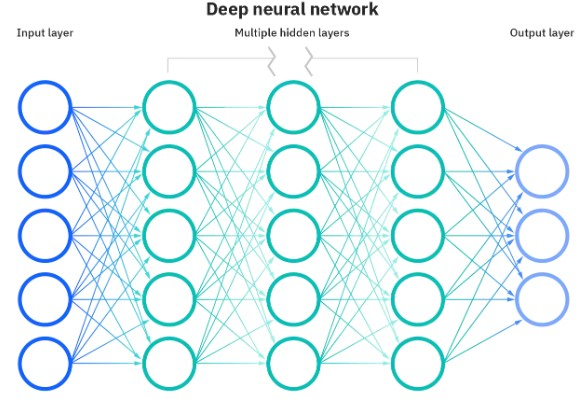
\includegraphics[height=.75\textheight]{images/deep_neural_network.jpg}
    \end{figure}
\end{frame}

\begin{frame}{Annexe : exemples de fonctions d'activations}
    \begin{figure}
    \centering
        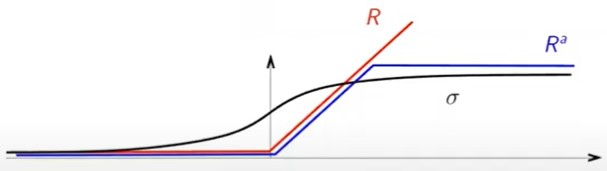
\includegraphics[width=\textwidth]{images/activations.jpg}
    \end{figure}
    En rouge, RELU, en bleu : RELU saturée, en noir la sigmoïde avec norme inf. de la dérivée inférieure à $1$.
\end{frame}

\begin{frame}{Annexe : exemples de courbes d'apprentissage}
\begin{columns}[t]
    \begin{column}{0.49\textwidth}
        \centering
        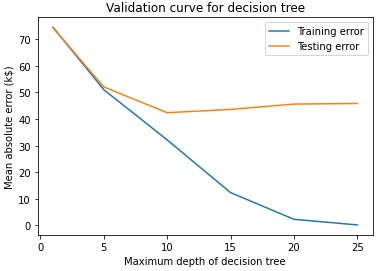
\includegraphics[width=\textwidth]{images/validation_curves.jpg}
    \end{column}
    \begin{column}{0.49\textwidth}
        \centering
        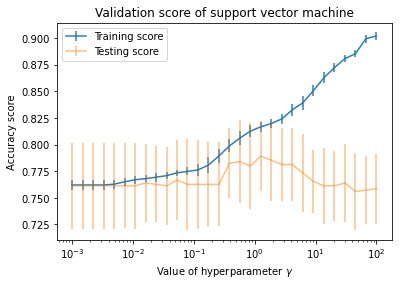
\includegraphics[width=\textwidth]{images/validation_score.jpg}
    \end{column}
\end{columns}
\end{frame}

\begin{frame}{Annexe : exemple de rapport d'apprentissage pour la sélection de modèles}
    \begin{figure}
        \centering
        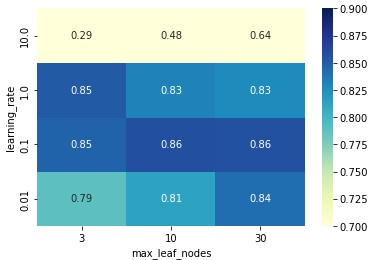
\includegraphics[width=\textwidth]{images/selection_modele.jpg}
    \end{figure}
\end{frame}

\end{document}
